\documentclass{article}
\usepackage{graphicx}
\usepackage{subcaption}

\title{Report 8: Scatter Pattern - RGB to HSV Conversion}
\author{Nam Le}
\date{\today}

\begin{document}

\maketitle

\section{Implementation}
I implemented the Scatter pattern for data layout conversion between Array of Structs (AoS) and Struct of Arrays (SoA) based on Slides 10--13:
\begin{enumerate}
    \item \textbf{RGB2HSV Kernel (Scatter)}: Converted the 3D RGB image (AoS) into three separate 2D device arrays \texttt{outH}, \texttt{outS}, and \texttt{outV} (SoA) using the formulas in Slide 12.
    \item \textbf{HSV2RGB Kernel (Gather/Scatter)}: Reconstructed the RGB image (AoS) from the three HSV component channels (SoA) according to the 6 angular regions defined in Slide 13.
\end{enumerate}

\section{Experimental Results}
The execution time was benchmarked across three 2D block size configurations: $(8, 8)$, $(16, 16)$, and $(32, 32)$.

\begin{figure}[h]
    \centering
    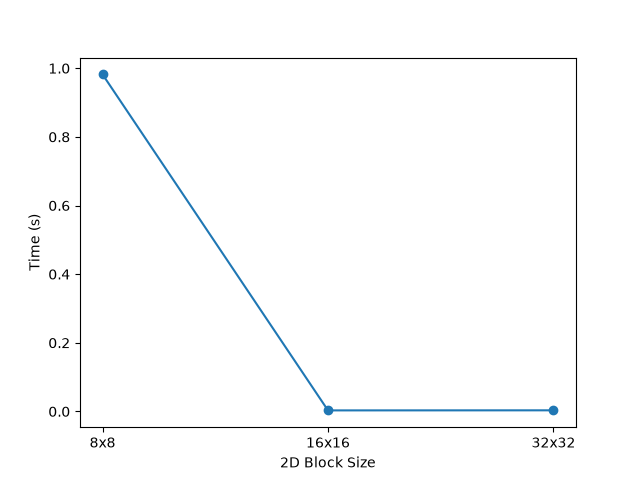
\includegraphics[width=0.7\textwidth]{scatter_block_size_vs_time.png}
    \caption{2D Block Size vs Total Execution Time for Labwork 8}
\end{figure}

\begin{figure}[h]
    \centering
    \begin{subfigure}[b]{0.45\textwidth}
        
\includegraphics[width=\textwidth]{input.jpg}
        \caption{Original Image}
    \end{subfigure}
    \hfill
    \begin{subfigure}[b]{0.45\textwidth}
        
\includegraphics[width=\textwidth]{reconstructed.jpg}
        \caption{Reconstructed Image}
    \end{subfigure}
    \caption{Input vs Reconstructed Output Image}
\end{figure}

\section{Discussion}
\begin{itemize}
    \item The reconstructed output image is visually identical to the original input image, confirming the mathematical correctness of both transformation kernels.
    \item Block size $(8, 8)$ took approximately $0.98$ seconds due to low thread occupancy per SM.
    \item Larger block dimensions like $(16, 16)$ and $(32, 32)$ significantly reduced execution time to near $0.001$ seconds, achieving better warp alignment and GPU memory bandwidth utilization.
\end{itemize}

\end{document}
